\documentclass{beamer}
\pdfstringdefDisableCommands{%
  \def\\{}%
  \def\texttt#1{<#1>}%
}
\beamertemplatenavigationsymbolsempty


% Footnote
\setbeamertemplate{footline}{\leavevmode%
  \begin{beamercolorbox}[wd=.33\paperwidth,left,ht=2.5ex,dp=1.5ex,rightskip=4pt plus 1pt, leftskip=4pt]{subsection in head/foot}
    Team 12
  \end{beamercolorbox}%
  \begin{beamercolorbox}[wd=.33\paperwidth,center,ht=2.5ex,dp=1.5ex]{section in head/foot}
  \end{beamercolorbox}%
  \begin{beamercolorbox}[wd=.34\paperwidth,ht=2.5ex,dp=1.5ex,leftskip=4pt plus 1pt,rightskip=4pt plus 1pt]{subsection in head/foot}
    \hfill\insertframenumber/\inserttotalframenumber
  \end{beamercolorbox}%
}


\title{Stato di avanzamento}
\subtitle{Sprint 1}
\author{
  \texorpdfstring{\parbox{45mm}{\centering\scriptsize Zaid Cheikh Ibrahim \\[-0.3em] {\tiny PO Operativo}}}{} \and 
  \texorpdfstring{\parbox{45mm}{\centering\scriptsize Tian Cheng Xia \\[-0.3em] {\tiny Scrum master}}}{}\\[1em]
  \texorpdfstring{\parbox{45mm}{\centering\scriptsize Qun Hao Henry Lee \\[-0.3em] {\tiny Developer}}}{} \and 
  \texorpdfstring{\parbox{45mm}{\centering\scriptsize Manuel Paris \\[-0.3em] {\tiny Developer}}}{}\\
}
\institute{
  Corso di Ingegneria del Software\\
  Alma Mater Studiorum $\cdot$ Università di Bologna  
}
\date{31 ottobre 2022}


\begin{document}

{
\setbeamertemplate{footline}{} 
\begin{frame}
  \titlepage
\end{frame}
}
\addtocounter{framenumber}{-1}

\begin{frame}
  \frametitle{Obiettivi dello sprint}
  \begin{itemize}
    \item Overview delle API di Twitter
    \item Realizzare i primi meccanismi di ricerca dei tweet
    \item Implementare le prime funzionalità per l'analisi dei dati
  \end{itemize}
\end{frame}

\begin{frame}
  \frametitle{Use case}
  \begin{figure}
    \centering
    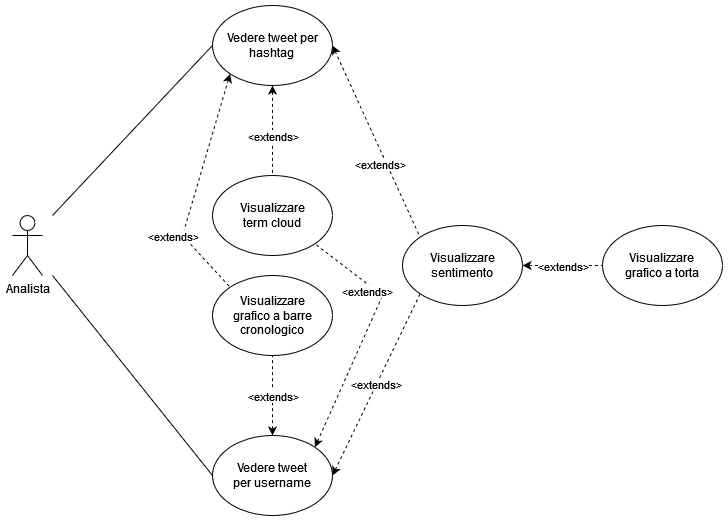
\includegraphics[width=\textwidth]{./img/usecase.png}
  \end{figure}
\end{frame}

\begin{frame}
  \frametitle{Pre-retrospettiva}
  \begin{figure}
    \centering
    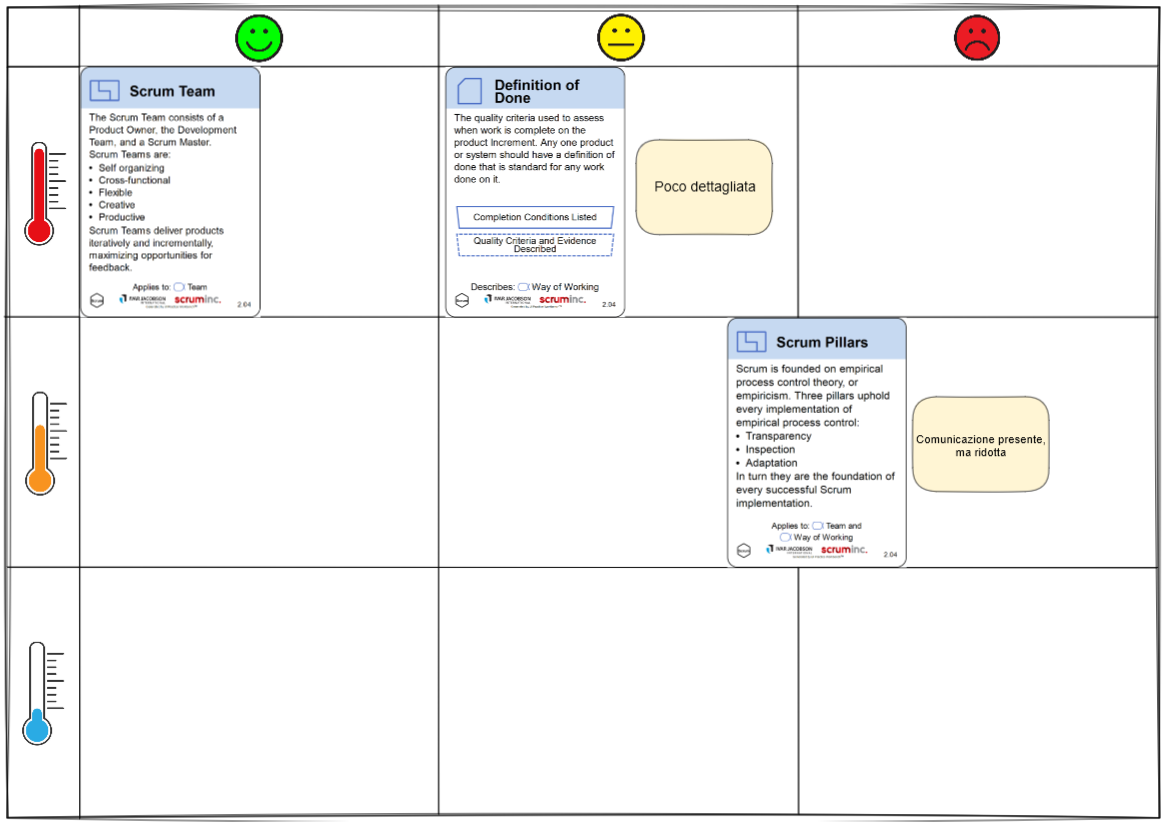
\includegraphics[width=\textwidth]{./img/essence.png}
  \end{figure}
\end{frame}

\begin{frame}
  \frametitle{Stato attuale}
  \begin{figure}
    \centering
    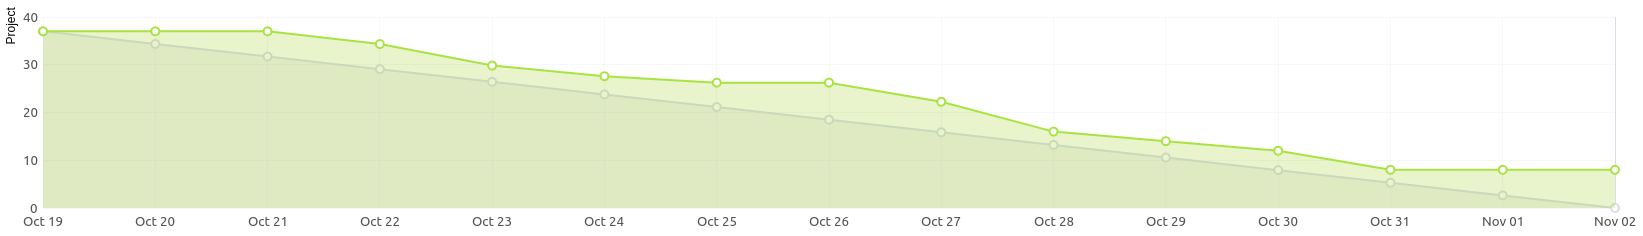
\includegraphics[width=\textwidth]{./img/burndown.png}
    \caption{Burndown chart}
  \end{figure}

  \begin{itemize}
    \item Ricerca di tweet per nome utente
    \item Analisi del sentimento di un tweet
  \end{itemize}
\end{frame}

\end{document}